%#BIBTEX bibtex Si$_3$N$_4$
\documentclass[twocolumn,amsmath,amssymb,a4paper,prb,superscriptaddress,floatfix]{revtex4-1}
\usepackage[dvipdfmx]{graphicx}
\usepackage{natbib}
\usepackage{multirow}
\usepackage{amsmath}
\usepackage{bm}
\usepackage{mathrsfs}
\usepackage{url}
\usepackage{color}
\usepackage{ulem}
\begin{document}

\title{First-principles calculation of lattice thermal
conductivities of $\alpha$-, $\beta$-, and $\gamma$-Si$_3$N$_4$}

\author{Kazuyoshi Tatsumi} \email{k-tatsumi@imass.nagoya-u.ac.jp}
\affiliation{Institute of
Materials and Systems for Sustainability, Nagoya University, Chikusa,
Nagoya 464-8603, Japan}
\affiliation{Center for Elements Strategy
Initiative for Structural Materials, Kyoto University, Sakyo, Kyoto
606-8501, Japan}

\author{Atsushi Togo}
\affiliation{Center for Elements Strategy Initiative for Structural
Materials, Kyoto University, Sakyo, Kyoto 606-8501, Japan}

\author{Isao Tanaka}
\affiliation{Center for Elements Strategy Initiative for Structural
Materials, Kyoto University, Sakyo, Kyoto 606-8501, Japan}
\affiliation{Department of Materials Science and
Engineering, Kyoto University, Sakyo, Kyoto 606-8501, Japan}
\affiliation{Nanostructures Research Laboratory, Japan Fine Ceramics
Center, Atsuta, Nagoya 456-8587, Japan}

\begin{abstract}
The lattice thermal conductivities of $\alpha$-, $\beta$- and $\gamma$-Si$_3$N$_4$
phases are investigated from {\it ab-initio} anharmonic lattice dynamics, within
the single-mode relaxation-time approximation of the linearized phonon Boltzmann
transport equation. At 300 K, the lattice thermal conductivity of
$\beta$-Si$_3$N$_4$ is calculated as $\kappa_{xx}=73$ and $\kappa_{zz}=199$ (in
units of W m$^{-1}$ K$^{-1}$), which is consistent with the reported experimental
values of 69 and 180, respectively. For $\alpha$-Si$_3$N$_4$, $\kappa_{xx}=68$
and $\kappa_{zz}=100$ are obtained.  The difference in anisotropy between these
phases originates from the characteristic differences in their phonon band
structures, which is closely related to the crystal structures.  In $\alpha$-Si$_3$N$_4$,
acoustic-mode phonons below 6 THz are the main heat carriers, while in
$\beta$-Si$_3$N$_4$, the phonon modes up to 12 THz contribute to the lattice
thermal conductivity. In $\gamma$-Si$_3$N$_4$, $\kappa=77$ is obtained. The
distribution of phonon mode contributions to the lattice thermal conductivity with
respect to phonon frequency closely resembles that for $\kappa_{xx}$
of $\beta$-Si$_3$N$_4$, although the phonon lifetimes for $\gamma$-Si$_3$N$_4$ are
twice as short as those for $\beta$-Si$_3$N$_4$.
\end{abstract}

\maketitle

\section{Introduction}
Several nitride insulators are known to exhibit high thermal conductivity, which
is important for heat transfer materials at elevated temperatures. For example,
Slack {\it et al.}\cite{slack} reported that wurtzite-type AlN has thermal
conductivity that exceeds 100 W m$^{-1}$ K$^{-1}$. Si$_3$N$_4$ has become another
promising thermal conductive insulator because its thermal conductivity has been
improved up to 177 W m$^{-1}$ K$^{-1}$ through the use of the advanced ceramic technologies
related to densification and microstructure
control.\cite{zhou,hirao-rev,watari,hirosaki} The Si$_3$N$_4$ ceramics
also exhibit high mechanical strength at elevated temperatures; therefore, they are
regarded as ideal materials for use in various applications, such as engine
components, gas turbines, and heat sink substrates of power semiconductor
devices.

At atmospheric pressure, Si$_3$N$_4$ has two phases, $\alpha$ and $\beta$, which
are generally considered as low- and high-temperature phases,
respectively.\cite{zhou,hirosaki-md,riley} Their crystal structures belong to
the P31c and P6$_3$/m space groups, respectively.\cite{yashima,boulay} These
structures have different manners of stacking equivalent basal layer structures
composed of SiN$_4$ tetrahedra.\cite{hampshire} Fig. \ref{fig:Fig1_cryst}
depicts these layer structures from the principal axis direction. They are
denoted as A, B, C, and D in the $\alpha$ phase, and A and B in the $\beta$
phase. The stacking manners are thus ABCDABCD... and ABAB..., respectively. The
$\alpha$ phase has additional two layer structures of C and D, which are related
to A and B by the $c$ glide operation.\cite{hampshire} Along this direction, the
lattice constant of the $\alpha$ phase is approximately twice as long as that of
the $\beta$ phase.
\begin{figure}[ht]
 \begin{center}
  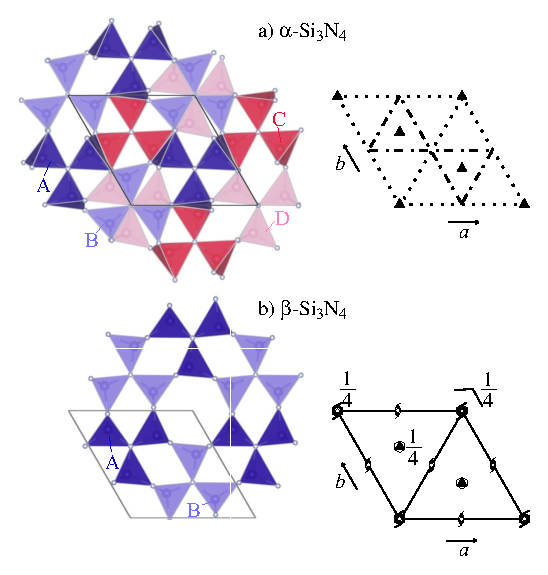
\includegraphics[width=0.90\linewidth]{Fig1_crystal_str2.eps} \caption{(color
  online) Crystal structures of $\alpha$- and $\beta$-Si$_3$N$_4$. Stacking of
  SiN$_4$ tetrahedron layers are shown at the left. (a) ABCDABCD... for
  $\alpha$-Si$_3$N$_4$. (b) ABAB... for $\beta$-Si$_3$N$_4$.  Space group
  diagrams\cite{inttableA} for P31c ($\alpha$-Si$_3$N$_4$) and P6$_3$/m ($\beta$-Si$_3$N$_4$)
  are shown at the right.}
  \label{fig:Fig1_cryst} 
 \end{center}
\end{figure}

The experimental thermal conductivities
\cite{zhou,hirao-rev,watari,hirosaki,hirai} of the Si$_3$N$_4$ polymorphs were
measured for the bulk polycrystalline samples. These values were significantly
affected by the lattice defects, impurities, shapes and orientations of the
constituent crystal grains;\cite{hirosaki-md} the intrinsic thermal conductivity
of defect-free Si$_3$N$_4$ has not been established. As an experimental approach
to determine this, Li {\it et al.}\cite{li} applied the high-resolution
thermoreflectance microscopy to single $\beta$-Si$_3$N$_4$ grains in a ceramic
sample. The thermal conductivity was analyzed as 69 and 180 W m$^{-1}$ K$^{-1}$
along the $a$ and $c$ axes, respectively.  These values respectively correspond
to the $xx$ and $zz$ elements of the lattice thermal conductivity tensor,
$\boldsymbol{\kappa}$. We consider the anisotropy of
$\kappa_{zz}/\kappa_{xx}\sim 3$ is relatively large. Hirosaki {\it et
al.}\cite{hirosaki-md} theoretically estimated $\boldsymbol{\kappa}$ by
application of the Green-Kubo formulation to the molecular dynamics (MD) method
with the interatomic potentials proposed by Vashishta {\it et
al.}\cite{vashishta}.  They calculated $\kappa$$_{xx}$ and $\kappa$$_{zz}$ of
$\alpha$-Si$_3$N$_4$ to be 105 and 225 W m$^{-1}$ K$^{-1}$, and those of
$\beta$-Si$_3$N$_4$ as 170 and 450 W m$^{-1}$ K$^{-1}$, respectively.  The ratio
$\kappa_{zz}/\kappa_{xx}$ in $\beta$-Si$_3$N$_4$ agreed well with the
experimental ratio; $\kappa_{xx}$ and $\kappa_{zz}$ were overestimated by more
than two times \textcolor{red}{that} of the experimental $\boldsymbol{\kappa}$. 

Based on first principles calculations and Boltzmann transport
theory\cite{phono3py}, Togo {\it{et al.}} recently calculated
$\boldsymbol{\kappa}$ of many polymorphs of the zincblende- and wurtzite-type
structures. Their crystal structures have stacking manners of the densest atom
planes as ABCABC... and ABAB..., respectively. The different stacking manners
merely altered $\boldsymbol{\kappa}$, the phonon linewidths and the phonon
density of states (DOS).\cite{phono3py} On the other hand, the previous MD
results indicated that the different stacking manners between the $\alpha$ and
$\beta$ phases altered $\boldsymbol{\kappa}$ significantly. This has not been
explained with respect to their phonon properties. Therefore, it is of interest
to investigate this based on the first principles anharmonic phonon calculation.

In addition to the $\alpha$ and $\beta$ phases, a cubic spinel phase
($\gamma$-Si$_3$N$_4$) is known to form upon compression and {\it{in situ}}
heating.\cite{zerr,zhang} The reported transition pressures are scattered from
10 to 36 GPa, depending on the experimental conditions.\cite{xu}  The $\gamma$
phase is experimentally quenched to atmospheric pressure and room temperature.
The thermal conductivity of the $\gamma$ phase has not been experimentally
reported, although it has been estimated by the Slack model.\cite{morelli} 

The present study aims to qualitatively elucidate the lattice thermal
conductivity tensors among the three Si$_3$N$_4$ phases by a first principles
approach.  We calculate $\boldsymbol{\kappa}$ of the $\gamma$ phase as well, for
systematic understanding. After the methodology section, we examine the validity
of the present results. The calculated thermal properties are then compared with
the available experimental and theoretical references.  The characteristic
behaviors of  $\boldsymbol{\kappa}$ are then investigated in detail on the basis
of the phonon band structures and phonon linewidths.

\section{Computational procedures}

\subsection{Lattice thermal conductivity calculation}

The lattice thermal conductivities were calculated by solving the linearized
Boltzmann transport equation (LBTE) within the single-mode relaxation time
approximation (single-mode RTA).  The harmonic phonon states and lattice thermal
conductivities were calculated with the phonopy\cite{phonopy} and
phono3py\cite{phono3py} software packages, respectively.  We also attempted the
direct-solution of LBTE\cite{chaput-direct} and give the calculated
$\boldsymbol{\kappa}$ values in the following section. The
\textcolor{red}{difference} between $\boldsymbol{\kappa}$ calculated by the
single-mode RTA and that by the direct solution was to be minor for our
discussion. Therefore, this research was limited to use the single-mode RTA to
take advantage of its \textcolor{green}{intuitive} closed form of
$\boldsymbol{\kappa}$.

In the following sections, we denote the phonon mode by $\lambda=(\mathbf{q},p)$
with the set of the phonon wave vector $\mathbf{q}$ and band index $p$ and
$-\lambda \equiv (-\mathbf{q},p)$. The relaxation time due to phonon-phonon
scattering was obtained as half the reciprocal of linewidth,
$\tau_{\lambda,\text{ph-ph}}=(2\Gamma_\lambda)^{-1}$, where the linewidth that was
employed is as follows:
\begin{align}
 \label{eq:linewidth}
 &\Gamma_\lambda = \frac{18\pi}{\hbar^2}
  \sum_{\lambda' \lambda''}
  \bigl|\Phi_{-\lambda\lambda'\lambda''}\bigl|^2 \times \nonumber \\ 
 &\left\{ (n_{\lambda'} + n_{\lambda''}+1) 
   \delta(\omega_\lambda-\omega_{\lambda'}-\omega_{\lambda''}) \right.
   + \nonumber \\ 
 &\;\;(n_{\lambda'}-n_{\lambda''})
  \left[\delta(\omega_\lambda +\omega_{\lambda'}-\omega_{\lambda''})
 \right. 
 \left. -\left. \delta(\omega_\lambda - \omega_{\lambda'}+\omega_{\lambda''})
 \right]\right\}.
\end{align}
Here, $\omega_\lambda$ is the harmonic phonon frequency of the phonon mode
$\lambda$, $n_\lambda=[\exp(\hbar\omega_\lambda/\mathrm{k_B}T)-1]^{-1}$ is
the Bose-Einstein distribution at temperature $T$, and
$\Phi_{\lambda\lambda'\lambda''}$ denotes the three-phonon-scattering strength.
$\Phi_{\lambda\lambda'\lambda''}$ was obtained by the usual coordinate
transformation of third-order force constants from direct space to phonon
space.\cite{phono3py} The second- and third-order real-space force constants
were obtained by {\it ab initio} calculation, of which the details are given in the
next section.

To more realistically compare the  calculated $\boldsymbol{\kappa}$ with the
measured thermal conductivities, the isotopic scattering effect due to the natural isotope
distribution was taken into account according to the second-order perturbation
theory.\cite{tamura} Using the relaxation times for the phonon-phonon scattering
and isotopic scattering, $\tau_{\lambda,\text{ph-ph}}$ and
$\tau_{\lambda,\text{iso}}$, respectively, the total relaxation time for a phonon mode,
$\tau_{\lambda}$, was calculated by assuming Matthiessen's rule, 
$1/\tau_{\lambda} = 1/\tau_{\lambda,\text{ph-ph}} +
1/\tau_{\lambda,\text{iso}}$.

The experimental thermal conductivities in the Si$_3$N$_4$ system were
measured for the polycrystalline samples and not from single
crystals. The conductivities measured in a polycrystalline area were affected
by various lattice defects within that area, such as grain boundaries, impurities, and
vacancies. We crudely took them into account by the relaxation time
$\tau_{\lambda,\text{bs}}=L/|\mathbf{v}_\lambda|$ of a phonon boundary
scattering model, where $\mathbf{v}_\lambda = \nabla_{\mathbf{q}}\omega_\lambda$
is the group velocity and $L$ is a parameter related to the boundary mean free
path. We consider $\tau_{\lambda,\text{bs}}$ as a variable parameter and partly
include it in the calculated $\boldsymbol{\kappa}$, according to Matthiessen's rule. 

The closed form of $\boldsymbol{\kappa}$ within the RTA was obtained via
\begin{align}
 \label{eq:kappa}
 \boldsymbol{\kappa}(T) = \frac{1}{N_\mathbf{q}\Omega} \sum_\lambda
 \tau_\lambda(T) \mathbf{v}_\lambda \otimes \mathbf{v}_\lambda c_\lambda(T),
\end{align}
where $N_\mathbf{q}$ is the number of
$\mathbf{q}$-points, $\Omega$ is the unit cell volume, and $c_\lambda$
is the mode heat capacity. To analyze $\boldsymbol{\kappa}$ in detail, 
the cumulative thermal conductivity:
\begin{align}
 \label{eq:cum-kappa}
 \boldsymbol{\kappa}^\text{c}(\omega) = \frac{1}{N_\mathbf{q}\Omega}
 \int_0^\omega \sum_\lambda
 \tau_\lambda(T) \mathbf{v}_\lambda \otimes \mathbf{v}_\lambda
 c_\lambda(T) \delta(\omega'-\omega)d\omega',
\end{align}
and its derivative $\frac{\partial
\boldsymbol{\kappa}^\text{c}(\omega)}{\partial \omega}$, were calculated to
determine the phonon mode
contributions to $\boldsymbol{\kappa}$.

\subsection{Computational details}

The force constants required for the lattice dynamics were calculated using the
first-principles projector augmented wave method\cite{paw} (VASP
code\cite{vasp-1996,vasp-1995, vasp-1999}). The generalized gradient
approximation (GGA) parameterized by Perdew, Burke, and Ernzerhof\cite{pbe} was
used for the exchange correlation potential. A plane wave energy cutoff of 500
eV was employed. The crystal structures were optimized for 0 K and 0 GPa until
the residual forces acting on the constituent atoms were less than $10^{-6}$
eV\AA$^{-1}$. Here, the temperature and pressure were considered only for the
electronic system and the zero point lattice vibration was not considered. The
calculated lattice parameters were $a=7.808$ \AA and $c=5.659$ \AA for the
$\alpha$ phase, $a=7.660$ \AA and $c=2.925$ \AA for the $\beta$ phase, and
$a=7.787$ \AA for the $\gamma$ phase, which are in agreement with the experimental
data\cite{yashima,boulay,paszkowicz} within +0.7 \% error. The lattice volume
optimized with the local density approximation (LDA)\cite{lda} for the exchange
correlation potential was, for $\beta$-Si$_3$N$_4$, 3 \% smaller than the volume
optimized with GGA, which is a typical volume contraction of LDA. 
$\kappa_{xx}}$ and $\kappa_{zz}}$ calculated with LDA were larger by 0.3 and 2.6
\% than those calculated with GGA. For our discussion, these differences are
sufficiently small; therefore, the impact of the choice of exchange correlation
potential is considered to be minor in this study.

\begin{table}[ht]
	\caption{\label{table:LTC} Calculated lattice thermal conductivities 
 of $\alpha$-, $\beta$-, and $\gamma$-Si$_3$N$_4$
 (WK$^{-1}$m$^{-1}$) at 300 K with respect to several combinations of
 supercell sizes.}
 \begin{ruledtabular}
  \begin{tabular}{ccccc}
   \multirow{2}{*}{Phase}
   & \multicolumn{2}{c}{Supercell (\# of atoms)} &
   \multicolumn{2}{c}{LTC} \\
   \cline{2-5}
   & $3^\text{rd}$ force constants & $2^\text{nd}$ force constants & $xx$ & $zz$ \\
   \hline
   \multirow{6}{*}{$\alpha$}
   & $1\times 1\times 1$ (28) & $1\times
   1\times 1$ (28) & 37 &   57 \\ 
   & $1\times 1\times 2$ (56) & $1\times
   1\times 2$ (56) & 41 &   79 \\ 
   & $1\times 1\times 1$ (28) & $2\times
   2\times 2$ (224) & 55 &   81 \\ 
   & $1\times 1\times 2$ (56) & $2\times
   2\times 2$ (224) & 67 &   95 \\ 
   & $1\times 1\times 2$ (56) & $2\times
   2\times 3$ (336) & 68 &  97 \\ 
   & $1\times 1\times 2$ (56) & $3\times
   3\times 4$ (1008) & 68 &  100 \\ 
   \hline
   \multirow{5}{*}{$\beta$}
   & $1\times 1\times 2$ (28) & $1\times
   1\times 2$ (28) & 44 & 173 \\ 
   & $1\times 1\times 2$ (28) & $2\times
   2\times 4$ (224) & 76 &  208 \\ 
   & $1\times 1\times 3$ (42) & $2\times
   2\times 4$ (224) & 71 & 194 \\ 
   & $1\times 1\times 3$ (42) & $2\times
   2\times 5$ (280) & 72 & 196 \\ 
   & $1\times 1\times 3$ (42) & $3\times
   3\times 8$ (1008) & 73 & 199 \\ 
   \hline
   \multirow{3}{*}{$\gamma$}
   & $1\times 1\times 1$ (56) & $1\times
   1\times 1$ (56) & \multicolumn{2}{c}{72} \\ 
   & $1\times 1\times 1$ (56) & $2\times
   2\times 2$ (448) & \multicolumn{2}{c}{77} \\ 
   & $1\times 1\times 1$ (56) & $3\times
   3\times 3$ (56) & \multicolumn{2}{c}{79} \\ 
  \end{tabular}
 \end{ruledtabular}
\end{table}

The force constants were calculated by the finite difference
approach\cite{wei-supercell}. For this calculation, the following supercells
were adopted: $1\times 1\times2$, $1\times 1\times3$, and $1\times 1\times1$
supercells of the conventional unit cells for the calculations of the
third-order force constants of $\alpha$, $\beta$, and $\gamma$-Si$_3$N$_4$,
respectively, and $3\times 3\times4$, $3\times 3\times8$ and $2\times 2\times2$
for those of the second-order force constants.  The length of the induced atomic
displacements was set to 0.03 \AA.  Table \ref{table:LTC} shows
$\boldsymbol{\kappa}$ calculated with several different sets of the supercells,
which indicates that the calculated $\boldsymbol{\kappa}$ has reasonable
convergence with respect to the size of the supercells. 

Uniform $\mathbf{k}$-point sampling meshes of $4\times 4\times 2$, $4\times
4\times 3$, and $3\times 3\times 3$ were employed for calculations of the
third-order force constants of the $\alpha$, $\beta$, and $\gamma$ phases. For
the $\alpha$ and $\beta$ phases, the center of the $a^*b^*$ plane was sampled,
while the center on the $c^*$-axis was not. For the $\gamma$ phase, a non-$\Gamma$
center mesh was used. For the calculations of the second-order force constants,
the $\Gamma$-point was only sampled for the $\alpha$ and $\beta$
phase\textcolor{red}{s}, and the
only one $\mathbf{k}=(0.5, 0.5, 0.5)$ point was sampled for the $\gamma$ phase.
The $\mathbf{q}$-point sampling meshes of $10\times 10\times 14$, $10\times
10\times 26$, and $12\times 12\times 12$ were employed to calculate
$\boldsymbol{\kappa}$ in Eq.~(\ref{eq:kappa}) for the $\alpha$, $\beta$, and
$\gamma$ phases, respectively.

Non-analytical term correction\cite{wang} was applied to the second-order force
constants to take into account the long range coulombic forces present in ionic
crystals. For the correction, static dielectric constants and Born effective
charges were calculated using the density functional perturbation theory
as implemented in the VASP code\cite{vasp-lepsiron,lepsiron}.

The effect of lattice thermal expansion on $\boldsymbol{\kappa}$ was examined
by the calculation of $\boldsymbol{\kappa}$ for several finite
temperatures with the crystal structures optimized for the
corresponding temperatures within the quasi-harmonic approximation
(QHA)\cite{dove-p76}. These $\boldsymbol{\kappa}$ were different from those
calculated for the same temperatures with the structure
optimized for 0 K. We consider these differences as the effect of lattice
thermal expansion. \textcolor{red}{The differences in $\boldsymbol{\kappa}$ for $T$=300, 600,
900, 1200, and, 1500 K, for the $\beta$ phase, were within 1 \%. The magnitude
was similar to that for Si and Ge calculated by Ward {\it{et
al.}}\cite{ward-ltc}.} 
%Similar differences in $\boldsymbol{\kappa}$ for $T$=300,
%600, 900, 1200, and, 1500 K within 1 \% were determined in the case of Si and
%Ge\cite{ward-ltc}. 
For the present study, these differences are negligible and
for finite temperatures $\boldsymbol{\kappa}$ calculated with the
structure optimized for 0 K was adopted.


The volumetric thermal expansion coefficients were also calculated. 
\textcolor{red}{Comparison with the experimental coefficient is useful to validate the present
thermal conductivity calculation because both the thermal expansion
and $\boldsymbol{\kappa}$ originate from the anharmonicity of the interatomic
potential.}
%Comparison with the experimental coefficients is useful to validate the present
%thermal conductivity calculation because the thermal expansion originates
%from both the anharmonicity of the interatomic potential and
%$\boldsymbol{\kappa}$. 
The calculated coefficients of the $\alpha$, $\beta$, and $\gamma$ phases were
4.31$\times 10^{-6}$,  4.19$\times 10^{-6}$, and 1.13$\times 10^{-5}$
K$^{-1}$
for 300 K, while the experimental values\cite{minikayev-alpha, gamma-expand}
were 3.75$\times 10^{-6}$ , 3.55$\times 10^{-6}$, and 9.48$\times
10^{-6}$ K$^{-1}$. The calculation systematically overestimated the experimental
values, but reproduced the experimental tendencies, including that the $\alpha$
phase has a slightly larger thermal expansion coefficient than the $\beta$
phase. This supports the validity of the present calculation to qualitatively
compare the calculated $\boldsymbol{\kappa}$ among the Si$_3$N$_4$ phases.

To compare the microscopic phonon properties among the three phases under the
same conditions, the results calculated at 0 GPa are shown and discussed.  For
the $\gamma$ phase, this means that we assume the condition of a virtually
quenched $\gamma$ phase at 0 GPa from the high pressure. To examine the
analytical continuity of the properties with respect to pressure,
$\boldsymbol{\kappa}$ of the $\gamma$ phase was calculated at 10, 20, and 40
GPa, as shown in Fig.~\ref{fig:S1}. The phenomenological behavior of the linear
dependence of $\boldsymbol{\kappa}$ with respect to the pressure was reproduced,
similar to that in Ref.~\onlinecite{andersson-pressure}. The slope was 2.89
W m$^{-1}$ K$^{-1}$ GPa$^{-1}$ for the $\gamma$ phase.  From this dependence, we
consider that the microscopic values are also varied smoothly with the pressure
and those at 0 GPa are valuable for comparison with the corresponding values of
the $\alpha$ and $\beta$ phases.

\subsection{Direct solution of LBTE}

The advantage of employing the single-mode RTA for thermal conductivity
calculations is the closed form, by which the qualitative character of
$\boldsymbol{\kappa}$ can be intuitively understood in terms of the phonon-mode
specific properties. The microscopic understanding of the full solution of LBTE
is still under development,\cite{cepellotti-relaxons} and the microscopic
picture based on collective phonons\cite{hardy-collective} will require more
complicated investigation.

Single-mode RTA solutions of LBTE often underestimate the full
solution.\cite{mukhopadhyay-ltc,ward-ltc} To check this underestimation,
$\boldsymbol{\kappa}$ for the $\alpha$ and $\beta$ phases were calculated by the
direct solution of LBTE\cite{chaput-direct}, which is one of the methods of LBTE
full solutions. $\kappa_{xx}$ and $\kappa_{zz}$ without the isotope effect were
69 and 102 W m$^{-1}$ K$^{-1}$ for the $\alpha$ phase, and 76 and 238
W m$^{-1}$ K$^{-1}$ for the $\beta$ phase, respectively, while the corresponding
single-mode RTA values were 70 and 102 W m$^{-1}$ K$^{-1}$ for the $\alpha$ phase,
and 76 and 210 W m$^{-1}$ K$^{-1}$ for the $\beta$ phase. $\kappa_{zz}$ for the
$\beta$ phase from the direct solution was 13 \% larger than that of the
single-mode RTA solution. The differences in $\boldsymbol{\kappa}$ between the
LBTE solutions are not significant; therefore, we expect that the physics of
these lattice thermal conductivities can be well understood within the
single-mode RTA at the current level of our interest. Therefore, we discuss the
lattice thermal conductivities calculated by the single-mode RTA solution.

\section{Results and discussion}

\subsection{Lattice thermal conductivities}

\begin{table}[ht]
 \caption{\label{table:LTC-exp} Calculated thermal conductivities of
 $\alpha$-Si$_3$N$_4$ (trigonal), $\beta$-Si$_3$N$_4$ (trigonal), and
 $\gamma$-Si$_3$N$_4$ (cubic) at 300
 K in units of W m$^{-1}$ K$^{-1}$, compared with the experimental and theoretical
 reference data. Theoretical bulk moduli $B$ (in
 units of GPa), calculated using the present band
 method are presented in the fourth column.}

\begin{ruledtabular}
 \begin{tabular}{ccccccccc}
   & \multicolumn{3}{c}{This work} & \multicolumn{3}{c}{Ref. Theo.}
   & \multicolumn{2}{c}{Ref. Expt.} \\
   \cline{2-9}
   & $\kappa_{xx}$ & $\kappa_{zz}$ & $B$ & $\kappa$ & $\kappa_{xx}$ & $\kappa_{zz}$ & $\kappa_{xx}$ & $\kappa_{zz}$ \\
   \hline
   $\alpha$-Si$_3$N$_4$ & 68 & 100 & 224 & 70\footnotemark[1] & 105\footnotemark[2] & 225\footnotemark[2] & - & -  \\
   $\beta$-Si$_3$N$_4$ & 73 & 199 & 237 & 250\footnotemark[1] & 170\footnotemark[2] & 450\footnotemark[2] & 69\footnotemark[3] & 180\footnotemark[3] \\
   $\gamma$-Si$_3$N$_4$ & 77 & - & 296 & 80\footnotemark[1] & - & - & - & - 
   \footnotetext[1]{Ref.~\onlinecite{morelli}, Slack model.}
   \footnotetext[2]{Ref.~\onlinecite{hirosaki-md}, molecular dynamics (Green-Kubo).}
   \footnotetext[3]{Ref.~\onlinecite{li}, single crystalline grains of poly-crystals.}
  \end{tabular}
 \end{ruledtabular}
\end{table}

Table~\ref{table:LTC-exp} shows the calculated
$\boldsymbol{\kappa}$ for 300 K.  $\beta$-Si$_3$N$_4$ has a markedly more
anisotropic $\boldsymbol{\kappa}$ than $\alpha$-Si$_3$N$_4$.  The directional
averages $\sum_i \kappa_{ii}/3$  are 79, 115,  and 77 W m$^{-1}$ K$^{-1}$ for the
$\alpha$, $\beta$, and $\gamma$ phases, respectively. The value for the
$\gamma$ phase is similar to that for the $\alpha$ phase, despite the
comparatively large difference among the bulk moduli ($B$) that are also shown
in Table~\ref{table:LTC-exp}.   

Table~\ref{table:LTC-exp} also lists the previously reported
experimental\cite{li} and theoretical\cite{hirosaki-md} $\boldsymbol{\kappa}$
for references. The theoretical results\cite{morelli} of the Slack model, which
do not include the anisotropy in $\boldsymbol{\kappa}$, are shown as $\kappa$ in
Table~\ref{table:LTC-exp}. Compared to the $\boldsymbol{\kappa}$ from
MD\cite{hirosaki-md}, our $\boldsymbol{\kappa}$ for the $\beta$ phase has better
agreement with the experimental $\boldsymbol{\kappa}$.  Compared to $\kappa$
from the Slack model, our directional average $\sum_i \kappa_{ii}/3$ is also
much closer to the experimental average. 

Fig.~\ref{fig:Fig1_338} shows the theoretical $\boldsymbol{\kappa}$ for the
$\alpha$ and $\beta$ phases as a function of $T$, together with the reference
experimental data\cite{hirosaki,hirai}. The experimental thermal conductivities
for a series of temperatures were measured on polycrystalline areas
by the laser flash method. These thermal conductivities (denoted as
$\kappa_\mathrm{polycrystal}$) cannot be directly compared with the calculated
intrinsic $\boldsymbol{\kappa}$, because they are largely dependent on the
microstructure of the samples; they deviate from the simple directional
averages of the intrinsic $\kappa_{ii}$, depending on the shapes of the crystal
grains. We treated this effect using the parameter $0\le{w}\le{1}$ and fitting
the quantity $w\kappa_{xx} + (1-w) \kappa_{zz}$ to the experimental
$\kappa_\mathrm{polycrystal}$ by the least squares method. We regard this as
theoretical $\kappa_\mathrm{polycrystal}$. 

\begin{figure}[ht]
 \begin{center}
  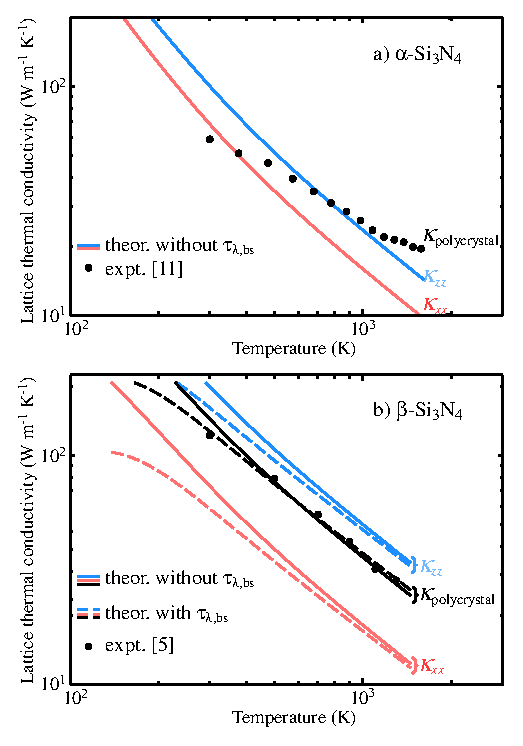
\includegraphics[width=0.90\linewidth]{Fig1_m1010.eps} \caption{(color
  online) Dependence of thermal conductivity on the temperature for $\alpha$- and
  $\beta$-Si$_3$N$_4$. For $\beta$-Si$_3$N$_4$, theoretical conductivities with the
  boundary scattering effect are shown by broken lines. Theoretical
  $\kappa_\mathrm{polycrystal}$ 
  (see text) for the $\beta$-Si$_3$N$_4$ sample are
  also shown for comparison with the experimental conductivities.}
  \label{fig:Fig1_338}
 \end{center}
\end{figure}

In Fig.~\ref{fig:Fig1_338}, $\kappa_{ii}$ calculated without
$\tau_{\lambda,\text{bs}}$ are almost proportional to $T^{-1}$ because
$n_\lambda$ in Eq.~(\ref{eq:linewidth}) can be reduced to
$\frac{\mathrm{k_B}T}{\hbar\omega_\lambda}-\frac{1}{2}$. In
Fig.~\ref{fig:Fig1_338}(a), the experimental $\kappa_\mathrm{polycrystal}$ of a
chemically vapor-deposited $\alpha$-Si$_3$N$_4$ sample\cite{hirai} is not
proportional to $T^{-1}$ and intersects the theoretical $\kappa_{ii}$. Thus, $w$
does not adjust the theoretical $\kappa_\rm{polycrystal}$ to the experimental
$\kappa_\rm{polycrystal}$.  The full solution of LBTE would negligibly cure the
disagreement.  Including the simple phonon lifetime of boundary scattering,
$\tau_{\lambda,\text{bs}}=L/|\mathbf{v}_\lambda|$, into the total phonon
lifetime could not explain the discrepancy either. A $L$ value of 0.6
$\mu\text{m}$, which was much smaller than the experimental grain
size\cite{hirai} of 10 $\mu\text{m}$, decreased the theoretical $\kappa$$_{ii}$
at the low temperature side toward the experimental valuesl; however,
$\kappa$$_{ii}$ at the high temperature side continued to be significantly
smaller than the experimental values. At present, the reason for the discrepancy
between the theoretical and experimental behavior is unclear. Although the
crystal structure of the experimental sample was characterized as
$\alpha$-Si$_3$N$_4$, significant lattice defects were present in the sample, as
pointed out by Hirosaki {\it et al.}\cite{hirosaki-md}, so that the simple
phonon boundary scattering model may fail to describe their effects on the
$\kappa_\mathrm{polycrystal}$. 

For the $\beta$ phase, the experimental $\kappa_\mathrm{polycrystal}$ is located
in-between the theoretical $\kappa$$_{xx}$ and $\kappa$$_{zz}$ curves, being
almost proportional to $T^{-1}$. Simple directional averages of the theoretical
$\kappa_{ii}$ slightly underestimate these experimental values. This is
understood from the control of the microstructure to increase
$\kappa_\mathrm{polycrystal}$, and the crystalline grains were selectively grown
along the $c$ axis of the most conductive direction.\cite{hirosaki} The
theoretical $\kappa_\mathrm{polycrystal}$ was fit well with $w=0.44$ to the
experimental. For the effects of lattice defects most of which were grain
boundaries, $\tau_{\lambda,\text{bs}}$ was included with $L=0.6$ $\mu\text{m}$
to further fit the theoretical curve ($w=0.33$) to the experimental data. $L$ is
slightly smaller than the average grain size\cite{hirosaki} of 2 $\mu\text{m}$
in the experiment; therefore, the discrepancy can presumably be explained by the
presence of other lattice defects than by the grain boundaries.


\subsection{Dispersion curves}

Fig.~\ref{fig:Fig4_ver5_338} shows phonon band diagrams for the three
Si$_3$N$_4$ phases. The branches are classified according to their symmetry
groups, using different colors and line styles. The solid and dashed lines are
used to represent degenerate and non-degenerate modes, respectively.
\textcolor{red}{The band diagrams on the other high-symmetry paths} are almost
identical to those reported earlier\cite{kuwabara,xu} and thus are not shown.
Here we investigate the frequency gradients, the group velocities projected on
the paths, with particular focus on their anisotropy in the $\alpha$ and $\beta$
phases. This was not investigated in the previous works.

\begin{figure}[ht]
 \begin{center}
  \includegraphics[width=0.90\linewidth]{Fig4_ver5_338_resize2_woDOS_color_simplified.eps}
    \caption{(color online) Calculated phonon band
		      diagrams (top) for three Si$_3$N$_4$ phases and Brillouin-zones (bottom).
  \label{fig:Fig4_ver5_338} }
 \end{center}
\end{figure}

The $\alpha$ phase unit cell contains two times more basal layer
structures than the $\beta$ phase unit cell; therefore, the edge of the $\alpha$ phase
Brillouin zone in stacking direction A is half as far as that of the $\beta$
phase. The number of phonon branches in the $\alpha$ phase are twice 
that in the $\beta$ phase. Phonon branches that are adjacent in
frequency and belong to the same symmetry group generally show a band gap, and an
anticrossing occurs when they are close to each other. If we regard the $\alpha$ phase
lattice as a superlattice of the $\beta$ phase lattice, then the phonon branches
of the $\alpha$ phase in Fig.~\ref{fig:Fig4_ver5_338}(a) are produced by folding
the phonon branches of the $\beta$ phase at the perpendicular bisector plane of
$\Gamma$A. Taking for example the folding of the acoustic phonon branch, in
Fig.~\ref{fig:Fig4_ver5_338}(a), an upper branch that belongs to the same symmetry
group is located very close in frequency, which inevitably entails an anticrossing
and a band gap between them. This explains why the folded branch, which is
degenerate at A with the acoustic branch due to the non-symmorphic symmetry, can
not increase its frequency as it goes back on $\Gamma$A in
Fig.~\ref{fig:Fig4_ver5_338}(a). The band gap and anticrossings  are
reported in the theoretical study on the lattice thermal conductivities of GaAs/AlAs
superlattices.\cite{GaAs/AlAs} It is interesting that these effects occur in the
present system, due to the stacking manners of the unit structures composed of
the same elements.


As a result, in Fig.~\ref{fig:Fig4_ver5_338}(a), the acoustic phonon branches
increase their frequencies similarly between these paths. In contrast, the
corresponding frequencies in Fig.~\ref{fig:Fig4_ver5_338}(b) increase much more
from $\Gamma$ to A than from $\Gamma$ to K. The anisotropic frequency
increments indicate an anisotropic $\mathbf{v}_\lambda$. Compared with the
$\alpha$ and $\gamma$ phases, the $\beta$ phase shows significantly steep slopes
for the low frequency optical phonon branches on $\Gamma$A, which indicates that
 $\rm{v}_{\lambda,z}$ of these phonon modes are large. The anisotropic
$\mathbf{v}_\lambda$ of the acoustic and low-frequency optical phonons will be
investigated further in the following sections. 

In the $\gamma$ phase, the longitudinal acoustic branches maintain linear
dispersion at higher frequencies than in the other phases. The gradients of
$\omega_\lambda$ for the $\gamma$ phase are the largest among the three phases,
as expected by the largest $B$.

\subsection{$\omega_\lambda$ contour map on the reciprocal plane}

\begin{figure}[ht]
 \centerins
  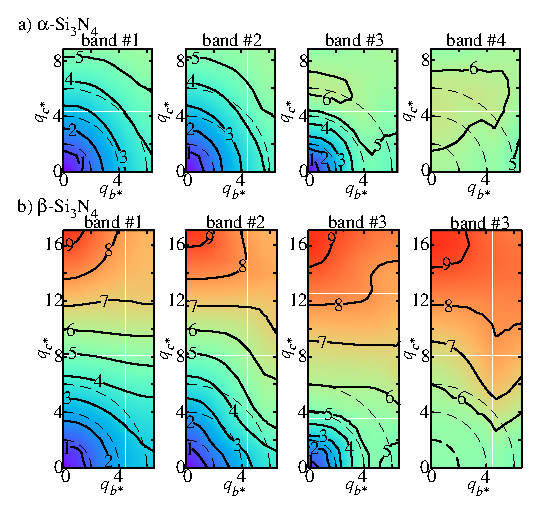
\includegraphics[width=\linewidth]{Fig2_small.eps} \caption{(color
  online) Contour maps of phonon frequency (THz) on the $b^*c^*$
  planes of Brillouin-zones. The coordinates in the reciprocal plane 
   are in units of $10^{-2}$ \AA$^{-1}$. The maps for the four lowest-frequency
  phonon modes are shown. The frequency landscapes are formed by simply
  connecting the frequencies of the same band indices, assigned in
  ascending order of frequency at the respective $\mathbf {q}$
  points. \label{fig:Fig3_338} }
 \centering
\end{figure}

We investigate the anisotropy in $\mathbf{v}_{\lambda}$ of $\alpha$- and
$\beta$-Si$_3$N$_4$ phases using another geometry, i.e., a cross-section of the
Brillouin-zone. Fig.~\ref{fig:Fig3_338} shows contour maps of
$\omega_{\lambda}$  on the $b^*c^*$ plane.  We show the maps for the four
lowest-frequency bands because they contribute significantly to 
$\boldsymbol{\kappa}$, which will be confirmed in the next section. There were
negligible differences between the distributions on the $b^*c^*$ plane and the
other planes containing the $c^*$ axis.  Therefore, the $b^*c^*$ plane was
selected as a
representative plane. In the $\alpha$ phase, the $\omega_{\lambda}$ distributions and
thus $\mathbf{v}_{\lambda}$ are almost isotropic. In the $\beta$ phase, the
contours are rather parallel to the $b^*$ axis, and thus the
$\mathbf{v}_{\lambda}$ tends to orient toward the $c^*$ axis direction. This
confirms the large anisotropy of $\mathbf{v}_{\lambda}$ 
of the acoustic and low-frequency optical phonon branches for the $\beta$ phase.

\subsection{Frequency distributions of phonon properties}

\begin{figure*}[ht]
 \begin{center}
	 \includegraphics[width=0.9\linewidth]{figure_dos_jdos_kc_m1010_dos_wo_arrows_bw.eps}
  \caption{(color online) Microscopic phonon properties of three Si$_3$N$_4$
	  phases. (a) Cumulative thermal conductivity $\boldsymbol{\kappa}^\text{c}$ and
	  its frequency derivative
	  , (b) DOS as $g(\omega)$, (c) DOS weighted with $\mathbf{v}_\lambda \otimes
	  \mathbf{v}_\lambda$ as $\boldsymbol{h}(\omega)$, and (d) scatter plots of
	  linewidths and phonon frequencies, $(\Gamma_\lambda,\omega_\lambda)$.
  \label{fig:Fig5_338_rev} }
 \end{center}
\end{figure*}

In the previous two sections, we have investigated the anisotropy in 
$\mathbf{v}_\lambda$, which may explain the anisotropy in
$\boldsymbol{\kappa}$. Here we examine which phonon frequencies and which terms
in the RTA closed form characterize the behavior of the present
$\boldsymbol{\kappa}$. In the following, we disregard the term of mode heat
capacity because it is approximately constant for 300 K.
For simplicity, the effects of isotope scattering and boundary scattering are not considered.
For the investigation, the cumulative thermal conductivity,
$\boldsymbol{k}^c(\omega)$ in Eq.(\ref{eq:cum-kappa}), and its
derivative $d\boldsymbol{\kappa}^c/d\omega$, are shown at the top of
Fig.~\ref{fig:Fig5_338_rev}. From this figure, it is evident that in the
$\alpha$, $\beta$, and $\gamma$ phases, the phonon modes with their frequencies
up to ca. 6, 12 and 10 THz largely contribute to each respective
$\boldsymbol{\kappa}$. The frequencies shown in the contour maps in
Fig.~\ref{fig:Fig3_338} are within these frequency ranges, and thus it is
confirmed
that these bands make a significant contribution to $\boldsymbol{\kappa}$.  


Assuming $\tau_\lambda$ and $\mathbf{v}_\lambda$ constant, then
$d\kappa_{ii}^c/d\omega$ ($ii$=$xx,zz$) are proportional to phonon density of
states (DOS)  
\begin{align}
 \label{eq:dos}
 g(\omega) = \frac{1}{N_\mathbf{q}\Omega}
 \sum_\lambda
 \delta(\omega-\omega_{\lambda}).
\end{align}
In this context we view $g(\omega)$ as frequency distributions of heat
carrier density.  Alternatively, assuming only $\tau_\lambda$ constant,
then $d\boldsymbol{\kappa}^c/d\omega$ is proportional to
\begin{align}
 \label{eq:wdos}
 \boldsymbol{h}(\omega) = \frac{1}{N_\mathbf{q}\Omega}
 \sum_\lambda
 \mathbf{v}_\lambda \otimes \mathbf{v}_\lambda
 \delta(\omega-\omega_{\lambda}),
\end{align}
from which we examine the impacts of both of the $\mathbf{v}_\lambda$ and heat carrier
density.  $g(\omega)$ and  $\boldsymbol{h}(\omega)$
are shown in
Figs.~\ref{fig:Fig5_338_rev}-b and c.  As for the frequency
variation of $\tau_{\lambda,ph-ph}$, phonon linewidths are shown as scatter
plots of $(\Gamma_\lambda,\omega_\lambda)$ in Fig.~\ref{fig:Fig5_338_rev}-d.

Comparing between the $\alpha$ and $\beta$ phases,  their linewidth
distributions are qualitatively similar, except for a striking difference below
$\sim$5 THz, which will be examined later. The markedly different
$d\kappa_{ii}^c/d\omega$ between the two phases are therefore ascribed to the
corresponding $h_{ii}$. Moreover, because the overall spectral shapes of
$g(\omega)$ are also similar between the two phases, the $\mathbf{v}_\lambda$
alone accounts for the different behaviors of the $d\kappa_{ii}^c/d\omega$. Thus
we conclude that the different anisotropy in $\boldsymbol{\kappa}$ is
qualitatively explained by the different $\mathbf{v}_\lambda$, due to the
folding effects of the band gaps and anticrossings. In contrast to this, in the
case of the zincblende and wurtzite structures, the group velocities are
suggested to be similar from their band structures\cite{phono3py}, because the
anticrossings are not created by the folding, as the optical branches are
located at much higher frequencies than in the present system. This
must result in the similar $\boldsymbol{\kappa}$ between these structures,
irrespective of the stacking manners. 

The $\gamma$ phase has much different  $g(\omega)$, $\boldsymbol{h}(\omega)$,
and, $\Gamma_\lambda$ from the others as expected from the large differences in
the crystal structure. The most significant difference is in its phonon
linewidths. Below $\sim$10 THz, they are approximately twice larger than those
of the other phases. We will examine this details later.  As a result, the
$d\kappa_{xx}^c/d\omega$ shows relatively low intensities.  Since the
longitudinal acoustic phonon branch increases its frequencies much, as we have
examined in the band diagram, $d\kappa_{xx}^c/d\omega$ rather gradually
attenuates as frequency increases, occasionally resembling to
$d\kappa_{xx}^c/d\omega$ of the $\beta$ phase.

It is left curious that the linewidths are similar between the $\alpha$ and
$\beta$ phases although the group velocities show marked differences between
them.  In analogy to Lindsay {\it et al.}\cite{Lindsay}, we can say that
$\Gamma_\lambda$ in the present form depends on the phase space for the
available two phonons, $\{\lambda', \lambda''\}$, and  also depends on
$|\Phi_{\lambda\lambda'\lambda''}|^2$. We examine these terms one-by-one. A
distribution of two-phonon configurations is represented as a joint density of
states (JDOS),
${D_2(\mathbf{q},\omega)}$,  
\begin{align}
 \label{eq:jdos}
 &D_2(\mathbf{q},\omega) = D_2^{(1)}(\mathbf{q},\omega) +  D_2^{(2)}(\mathbf{q},\omega)
\end{align}
where 
\begin{eqnarray*}
	D_2^{(1)} & = & \frac{1}{N_\mathbf{q}Z^2} \sum_{\lambda'\lambda''}\Delta(-\mathbf{q} + \mathbf{q'} + \mathbf{q''}) \nonumber \\
								   & \times & [\delta(\omega + \omega_{\lambda'} - \omega_{\lambda''}) + \delta(\omega - \omega_{\lambda'} + \omega_{\lambda''})],\\
	D_2^{(2)} & = & \frac{1}{N_\mathbf{q}Z^2} \sum_{\lambda'\lambda''}\Delta(-\mathbf{q} + \mathbf{q'} + \mathbf{q''}) \nonumber \\
								   & \times & \delta(\omega - \omega_{\lambda'} - \omega_{\lambda''}),
\end{eqnarray*}
with $\Delta$($\mathbf{x}$) giving 1 if $\mathbf{x}$ is a reciprocal lattice
vector and otherwise zero. $Z$ is the number of formula units in the primitive unit cell
and included as a scaling factor to compare JDOS for the structures with different
$Z$.  The equation of the linewidth in Eq.~(\ref{eq:linewidth}) contains terms
of $(n_{\lambda'}+n_{\lambda''}+1)$ and $(n_{\lambda'}-n_{\lambda''})$. Thus in
more rigorous study, instead of $D_2^{(1)}$ and $D_2^{(2)}$,  we should
employ weighted JDOS with these terms.  We firstly employ the JDOS in
Eq.~(\ref{eq:jdos}) to intuitively examine the similarity between the
linewidths of the $\alpha$ and $\beta$ phases. The weighted JDOS (WJDOS)
will be briefly shown later including that of the $\gamma$ phase. 

Fig.~\ref{fig:Fig6_338} shows frequency-functions of JDOS at several different
$\mathbf{q}$-points. They have very weak $\mathbf{q}$-point dependences. At the
low frequency region up to $\simeq$ 10 THz $D_2^{(1)}$ is dominant between the
two terms. The $D_2^{(1)}$ are similar between the phases.  In the present
Si$_3$N$_4$ system, the phonon modes of the acoustic and low-frequency optical
branches, which largely contribute to the $\boldsymbol{\kappa}$, are much fewer
than the other phonon modes.  The JDOS are mainly determined by the latter
majorities.
As in the band diagrams, the branches of the majorities are rather flat. Thus we
can approximately disregard in Eq.~(\ref{eq:jdos}) the dependences of the
$\omega_{\lambda'}$ and $\omega_{\lambda''}$ on the $\mathbf{q}'$ and
$\mathbf{q}''$.  In this case $D_2^{(1)}$ is simplified to the half part
($\omega \geq  0$) of the auto-correlation function of DOS. The DOS for both
of the $\alpha$ and $\beta$ phases in Fig.~\ref{fig:Fig5_338_rev}-a have a
frequency gap. The $D_2^{(1)}$ reflect this DOS feature, dropping suddenly
around 0 THz and showing a small shoulder around 5 THz, corresponding to the
width of the gap.  Because the gap is originated from the local modes of the
planer NSi$_3$ composing each of the $\alpha$ and $\beta$ crystal
structures,\cite{kuwabara} the $D_2^{(1)}$ are similar in these phases.  

\begin{figure}[ht]
 \centering
  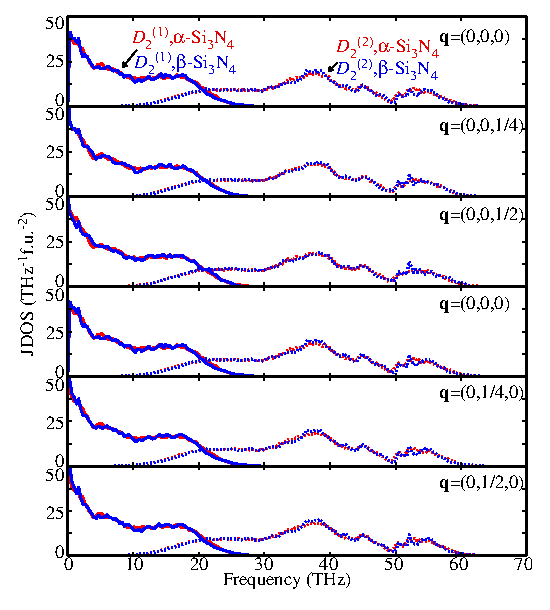
\includegraphics[width=0.9\linewidth]{figure_jdoss.eps} \caption{(color
	  online) JDOS of $\alpha$- and $\beta$-Si$_3$N$_4$ at different $\mathbf q$ points.
  The first and forth rows are JDOS at the same $\Gamma$-point but calculated
  with the polarization for non-analytic term correction set along $c^*$ and
  $b^*$, respectively. \label{fig:Fig6_338} }
 \centering
\end{figure}

The WJDOS are shown in Fig.~\ref{fig:Fig_wjdos}.  The terms corresponding to
$D_2^{(1)}$ and $D_2^{(2)}$ are denoted as $N_2^{(1)}$ and $N_2^{(2)}$. They are
weighted $D_2^{(1)}$ and  $D_2^{(2)}$ with $(n_{\lambda'}-n_{\lambda''})$ and
$(n_{\lambda'}+n_{\lambda''}+1)$, respectively. For the comparison among the
three phases, we only show the frequency distributions at $\mathbf{q}=(0,0,0)$
because the $\mathbf{q}$ dependences of the WJDOS were as weak as JDOS.  The
weighting factors reduce the $N_2^{(1)}$ near 0 THz and enhance the $N_2^{(2)}$
in the high frequency range.  The latter reduces the
$d\boldsymbol{\kappa}^c/d\omega$ in the high frequency range, for all the phases.
The total WJDOS are similar between the $\alpha$ and $\beta$ phases. The
$\gamma$ phase has slightly small intensities of the total WJDOS below $\sim$10THz.

\begin{figure}[ht]
 \centering
  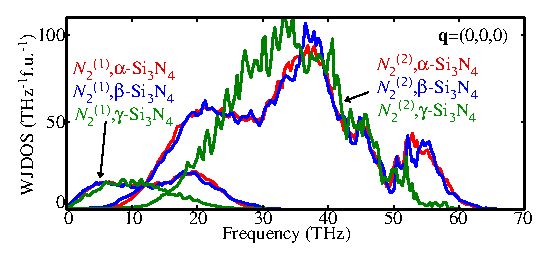
\includegraphics[width=0.9\linewidth]{Fig_wjdos.eps} \caption{(color
	  online) Comparison of WJDOS at $\mathbf{q}=(0,0,0)$ for 300 K among the three phases. 
		  } \label{fig:Fig_wjdos} 
 \centering
\end{figure}

\begin{table}[ht]
	\caption{\label{table:aveavepp} Averages of
	$|\Phi_{\lambda\lambda'\lambda''}|^2$ over frequency ranges of
	$\omega_\lambda$ (0--15 and 0--35 THz) and all ($\lambda'$,$\lambda'$). The
	values are in units of 10$^{-9}$ eV$^2$f.u.$^{2}$.}
 \begin{ruledtabular}
  \begin{tabular}{cccc}
	  \multirow{2}{*}{Frequency Range (THz)}
   & \multicolumn{3}{c}{Phase}  \\
   \cline{2-4}
   & $\alpha$ & $\beta$ & $\gamma$ \\
   \hline
   \multirow{1}{*}{0--15}
   & 1.1  &  1.1  & 2.3 &    
   \multirow{1}{*}{0--35}
   & 5.2 & 5.2 & 4.6 &     
  \end{tabular}
 \end{ruledtabular}
\end{table}

As for $|\Phi_{\lambda\lambda'\lambda''}|^2$, in Table.~\ref{table:aveavepp},
they are averaged over two kinds of frequency ranges of 0--15 or 0--35 THz for
$\omega_\lambda$ and all indices in $\lambda'$ and $\lambda''$.  The averages
are very similar values between the $\alpha$ and $\beta$ phases. With the
similar impacts of the (W)JDOS and $|\Phi_{\lambda\lambda'\lambda''}|^2$, the
linewidths in these phases are similar.  For the $\gamma$ phase, the large
$|\Phi_{\lambda\lambda'\lambda''}|^2$ attribute to the large linewidths.  We set
the frequency ranges for $\omega_\lambda$ so that the narrower frequency range
approximately corresponds to the range where the phonon modes largely contribute
to the $\boldsymbol{\kappa}$. A small change in the frequency ranges by a few
THz did not change the qualitative characters of the averages.  

\begin{figure}[ht]
 \centering
  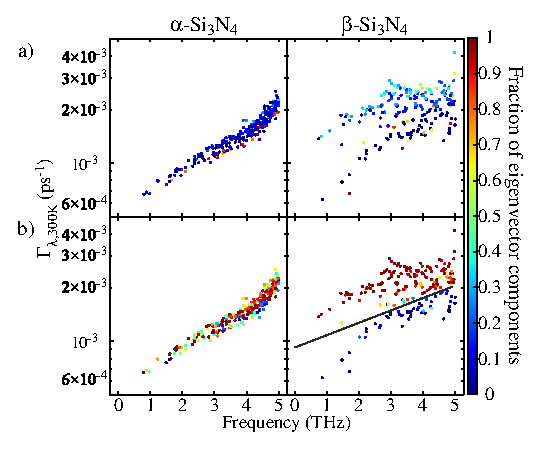
\includegraphics[width=\linewidth]{figure_analyze_gamma3_m1010_print.eps} \caption{(color
	  online) Distribution of linewidths $\omega_\lambda$ $\leq$ 5 THz
		  with colors with respect to strengths of eigenvector components along $\mathbf q$ (a)
		  and on $ab$ plane (b).} \label{fig:Fig7_338} 
 \centering
\end{figure}

Finally, we examine the exceptional, but striking difference in linewidth
distributions between the $\alpha$ and $\beta$ phases: In the $\alpha$ phase,
$\Gamma_\lambda$ below $\sim$5 THz are aligned on a single smooth line, while in
the $\beta$ phase, they are scattered roughly on two branches.  This difference
is investigated by trying to relate the linewidths with the directions of the
atomic vibrations of the phonon modes.  Fig.~\ref{fig:Fig7_338} enlarges the
$(\Gamma_\lambda,\omega_\lambda)$ plots in this frequency range. In
Fig.~\ref{fig:Fig7_338}-a, the $\Gamma_\lambda$ are classified using colors
according to the sums of the squares of the eigenvector components along the
$\mathbf{q}$; the sum is 1 for a perfectly longitudinal wave. However, these
sums show no clear contrast between the two branches in the $\beta$ phase.
Fig.~\ref{fig:Fig7_338}-b shows the same plot as Fig.~\ref{fig:Fig7_338}-a, but
with colors according to the sums of the squares of the eigenvector components
along the $ab$ plane, which is 1 when the eigenvector lays on the $ab$ plane.
There is a tendency in the $\beta$ phase that  $\Gamma_\lambda$ are large for
atomic vibrations along the $ab$ plane.  This means that the vibration modes
along the $ab$ plane, belonging to the acoustic phonon branches, are more easily
scattered in the $\beta$ phase, no matter whether they are longitudinal or
transverse. For the panel of $\beta$-Si$_3$N$_4$ in Fig.~\ref{fig:Fig7_338}-b, a
straight line splits the phonon modes to two groups. The numbers of the phonon
modes assigned to the larger and smaller $\Gamma_\lambda$ groups are 157 and 58,
whose ratio is confirmed close to the population ratio of the vibration modes
along and out of the $ab$ plane.


\section{Summary}

In the present study, we investigate the lattice thermal conductivities of the
three Si$_3$N$_4$ phases, by using the lattice dynamics based on the first
principles interatomic force constants. The main remarks are as follows:

1) In the $\alpha$- and $\beta$-Si$_3$N$_4$, whose crystal structures are
characterized by the stacking manners of the basal layer structures, which
largely alter $\boldsymbol{\kappa}$, due to the folding effects of the band gaps
and anticrossings. This contrasts with the case of
the zincblende and wurtzite structures in the previous study\cite{phono3py}.
The $\boldsymbol{\kappa}$ of $\alpha$-Si$_3$N$_4$ is rather isotropic, while the
$\kappa$$_{zz}$ of the $\beta$ phase is twice or more larger than the other
$\kappa_{ii}$ of the three phases.

2) In the $\alpha$ phase, the acoustic mode phonons below 6 THz are the main
heat carriers, while in the $\beta$ phase, the phonons below 12 THz contribute
to the $\boldsymbol{\kappa}$. Their group velocities are confirmed to characterize the
behaviours of $\boldsymbol{\kappa}$.

3) In the $\gamma$ phase, the frequency distribution of the phonon mode
contributions to $\boldsymbol{\kappa}$ is similar to that for $\kappa_{xx}$ of
$\beta$-Si$_3$N$_4$. Its large phonon-phonon scattering strength and steep
longitudinal acoustic branches attribute to this.



\section*{ACKNOWLEDGMENTS}
The present work was partly supported by Grants-in-Aid for Scientific
Research of MEXT, Japan (Grant No. 15K14108 and ESISM (Elements Strategy
Initiative for Structural Materials) of Kyoto University).

\appendix
\section{Pressure dependence of lattice thermal conductivity of $\gamma$-phase}
\begin{figure}[ht]
 \begin{center}
  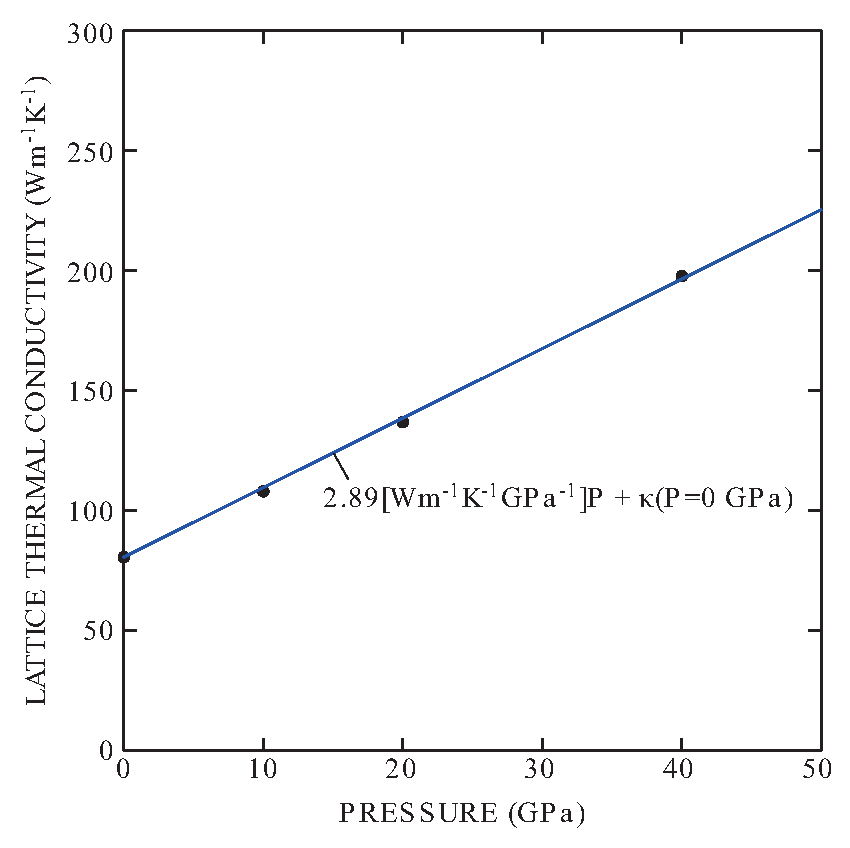
\includegraphics[width=0.80\linewidth]{S1.eps} \caption{(color online)
  Pressure dependence of lattice thermal conductivity of $\gamma$-Si$_3$N$_4$.  \label{fig:S1} }
 \end{center}
\end{figure}
\bibliography{Si3N4}
\end{document}
